\documentclass[conference]{IEEEtran}
\usepackage{url}
\usepackage{graphicx}
\usepackage{listings}
\usepackage{color}
\usepackage{fancyhdr}
\setcounter{topnumber}{8}
\setcounter{bottomnumber}{8}
\setcounter{totalnumber}{8}


%\onecolumn
% Title and Author Information
\title{Fall Detection Project - Master SSE - Hanze}

\author{\IEEEauthorblockN{
Ali Shirazi, Amir Masoud Jafari}

\IEEEauthorblockA{
a.shirazi@st.hanze.nl, a.jafari@st.hanze.nl}}

\date{March 2025}

\begin{document}

% Abstract
\maketitle

\thispagestyle{plain}
\pagestyle{plain}

\begin{abstract}
This document provides instructions on how to prepare a report about your project. This guideline includes basic information that is expected in a report, along with a suggested structure for how to organize it. Examples of how to include figures and tables in \LaTeX\, and a general style guide are also given. The usage of AI tools is also discussed. The text ends with a conclusion and a list of cited references.
\end{abstract}

\section{Introduction}

\noindent The project report is your final task in our journey to complete your project. It serves as a comprehensive documentation of your project work, highlighting your understanding of both the theoretical and practical aspects of design, implementation of your solution and analysis of the obtained results. 

Ensure that all team members contribute equally to the writing process, reflecting the collaborative effort invested in the project. The report should demonstrate your ability to design, implement, test, and evaluate the results of your project, presenting your findings in a professional format.


% Instructions Section
\section{Formatting Requirements}

\noindent You are free to write the report in \LaTeX\ or Word (a template is available for \LaTeX\ in Overleaf\footnote{\url{https://www.overleaf.com}}).  The report should adhere to the IEEE conference paper format, which is a two-column layout. The official IEEE template can be downloaded from the IEEE page\footnote{\url{https://www.ieee.org/conferences/publishing/templates.html}}. Following the formatting instructions in the template, all formatting shall be done automagically. Note, this guideline is also written in the IEEE template style. 


\section{Content Structure}
\label{sec:Content}

\noindent The report is structured to provide a comprehensive overview of the design and implementation process. Key sections include an introduction that outlines the context and problem being addressed, a literature review, a conceptual model (requirements, overview of the proposed solution, research question or goal), a detailed description of the design of the process to answer the research question (or to achieve the goal) and how to obtain and validate the results, results and discussion. Finally, the report concludes with a summary of findings and potential areas for improvement. To ensure reproducibility and transparency, code and other relevant information must be available and linked (for example, on GitHub). The suggested structure of your report is as follows. This structure is not set into stone, hence, you are free to adjust it to your needs. 


\begin{figure}[b]
  \centering
  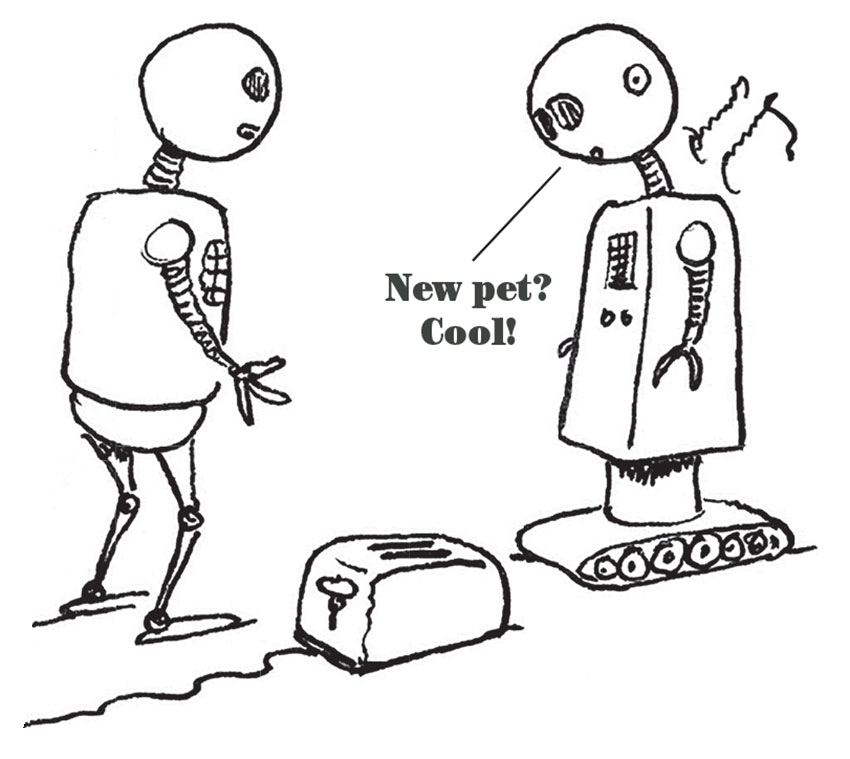
\includegraphics[width=0.7\columnwidth]{toasterpet.jpg}
  \caption{Comic by Scott Masear, adapted from \label{comic}\cite{joke}.}
\end{figure}


\begin{table*}
\centering
\caption{Example of a Table}
\label{tab:esp32_vs_rp2040}
\renewcommand{\arraystretch}{1.2} % Adjust row height for readability
\begin{tabular}{|l|c|c|}
\hline
\textbf{Feature} & \textbf{ESP32} & \textbf{RP2040} \\ \hline
\textbf{Manufacturer} & Espressif Systems & Raspberry Pi Foundation \\ \hline
\textbf{Core Architecture} & Xtensa Dual-Core (32-bit) & ARM Cortex-M0+ Dual-Core \\ \hline
\textbf{Clock Speed} & Up to 240 MHz & Up to 133 MHz \\ \hline
\textbf{RAM} & 520 KB SRAM & 264 KB SRAM \\ \hline
\textbf{Flash Memory} & Up to 16 MB (external SPI flash) & External flash via QSPI (no internal flash) \\ \hline
\textbf{GPIO Pins} & Up to 36 GPIO & Up to 30 GPIO \\ \hline
\textbf{Connectivity} & Wi-Fi, Bluetooth & None (requires external modules for connectivity) \\ \hline
\textbf{Peripherals} & 
UART, SPI, I2C, ADC, DAC, PWM, etc. & 
UART, SPI, I2C, ADC, PWM, PIO, etc. \\ \hline
\textbf{Power Consumption} & Moderate (Wi-Fi increases power use) & Low (optimized for low power) \\ \hline
\textbf{Development Ecosystem} & 
Arduino IDE, ESP-IDF, MicroPython & 
Arduino IDE, MicroPython, C/C++ SDK \\ \hline
\textbf{Price Range} & \$3–\$10 & \$1–\$4 \\ \hline
\end{tabular}
\end{table*}


\begin{itemize}
    \item \textbf{Title and Author Information}: Begin with the title of your project and your name(s) as the author(s). Include your university affiliation and email.
    \item \textbf{Abstract}: A brief summary of your report, not exceeding 200 words.  May be the last part to be written. The abstract should \underline{not} contain an introduction to the topic.
    \item \textbf{Keywords}: List 3–5 keywords that best describe your robot design and programming.
    \item \textbf{Introduction, Motivation}: Describe the background and importance of the topic, including relevant statistics and a specific description of the problem that you are addressing and the current situation. Context of company/research institute is important. List the requirements and possible ethical and environmental considerations. It may also be advisable to place a teaser figure (like Fig. \ref{comic}) right at the beginning of the paper, so that the reader becomes familiar with the topic more quickly. 
     \item \textbf{Literature Review}: Here you describe a few related works and compare state-of-the-art methods, including quantitative comparisons for key methods. Opportunities for improvement of methods or application are identified. Note that all literature used is referenced and listed at the end of the paper.
     \item \textbf{Conceptual Model}: Give an overview of the proposed solutions, list the corresponding requirements, and compare variants. Include a graphical overview of solution presented, like Figure \ref{schematic}. State the goal or the (S.M.A.R.T.) Research Question, and make sure to prioritize the sub-goals or sub-questions. 
    \item \textbf{Design}: Step-by-step approach to answer the Research Question or achieve the goal. Describe each step with evaluation/validation methods. Ethical/Environmental aspects are taken into consideration. Include a section on how to validate results. It is always a good idea to include figures to help with the understanding.
    \item \textbf{Results}: This section provides experimental data with a qualitative analysis, supported by illustrations. Results should be presented in the same order as the design. Figures must be cited and explained in the text, and must have captions with a concise description. Graphs must contain proper scale and units. 
    \item \textbf{Discussion}: Interpret and analyze your results, compare them to existing literature, explain unexpected results, acknowledged limitations of the setup.
    \item \textbf{Conclusion}: Summarize the main findings, discuss the significance of the study, answer the Research question / goals, evaluate the fulfillment of the requirements, and present suggestions for future research.
    \item \textbf{Acknowledgments}: help from other persons, like funding, proof-reading, and ideas or results adopted from other sources should be acknowledged.
    \item \textbf{Contributions}: For each author, itemize the contributions to the project, e.g. which sections have been written, which parts implemented, etc.     
    \item \textbf{References}: List all sources cited (and only the ones cited) in the text.
\end{itemize}

\section{Submission Guidelines}
\begin{itemize}
    \item \textbf{File format}: Submit your report as a \textbf{PDF file}.
    \item \textbf{Naming convention}: Name the file as: \\\texttt{YourGroupnumber\_Report.pdf}.
    \item \textbf{Length}: maximum 6 pages
    
\end{itemize}

\section{Usage of AI Tools}

\noindent You are permitted to use AI tools to assist in the preparation of your project report, but their use is strictly limited to reformatting and rephrasing text. You can also use such tools to assist in coding (like CoPilot). These tools should not be employed for generating content or ideas, as the report must reflect your original work and understanding. If you choose to use an AI tool, you are required to declare which model(s) was(were) used and explicitly specify the sections where it was applied. This ensures transparency and adherence to academic integrity. Failure to disclose the use of AI tools may result in penalties, so be diligent and honest in documenting their use.

The report must not contain any plagiarism, not even as modified text. 


\section{Style Guide}

\subsection{Bibliography}

\noindent \LaTeX\  offers its own environment for creating bibliographies. Make use of it! As literature sources,
only peer-reviewed publications, books, and technical reports are appropriate. These are papers with
authors, title and publication date, for journals with volume/number, for conferences optionally with
conference date and location. You may also name the publisher and page numbers, optionally a URL.
Examples for proper references are \cite{Dyn87,Far02,Lev44,Mar63}.


\subsection{Web Links}
\noindent Web links, blogs, etc. do not count as literature, since the internet is subject to continuous change
and its contents have not gone through a professional reviewing process.
Online-sources can either be listed separately, or be added to the text as footnotes.

\subsection{Professional Style}

\noindent The style of writing for scientific papers is focused and factual, without
digress (no "marketing", no jokes, no "sloppy" language).
The "I" form (and also the imperative, except for exercises) should be avoided.
You can use the "we" form if you are writing in a way that includes the reader
(also when you are the sole author, e.g. when writing a thesis).
As a rule, almost everything is written in present tense. If at all, the future tense is used in the last section.
The past tense can be used when dating related work.

\subsection{Figures, Tables, Equations}

\noindent It is important that figures and tables (flow objects created by LaTeX
placed at the top of the page) are provided with numbers and captions containing a meaningful description.

Each of these objects should be referenced (at least once) within the text where it is relevant.
The same applies to literature: every reference should appear at least once, including
one or two sentences dedicated to it. When working with BibTeX, only
those references that are used appear, at all. This way one can re-use the same literature base for multiple papers.

Equations are automatically numbered in round brackets by LaTeX, and this number is used when you make references to the equation using its label (just like Figures). The numbering of equations is very helpful for sharing when writing between multiple authors and reviewers. Equations are considered part of the text, so they must contain punctuation marks when applicable. Besides, all its variables need to be explained in the text. 

An example is the calculation of the current through the LED connected to pin 1 of the ESP32 in the circuit illustrated by Figure \ref{Fig:schematics}. The current $I_{LED}$ is calculated as

\begin{equation}
I_{LED} = \frac{V_{R}}{R},
\label{eq:ohm}
\end{equation}

\noindent where $V_{R}$ is the voltage across the $10 {\Omega}$ resistor connected in series with the LED, and $R$ is its resistance value. Equation (\ref{eq:ohm}) is known as Ohm's Law.


\begin{figure}
  \centering
  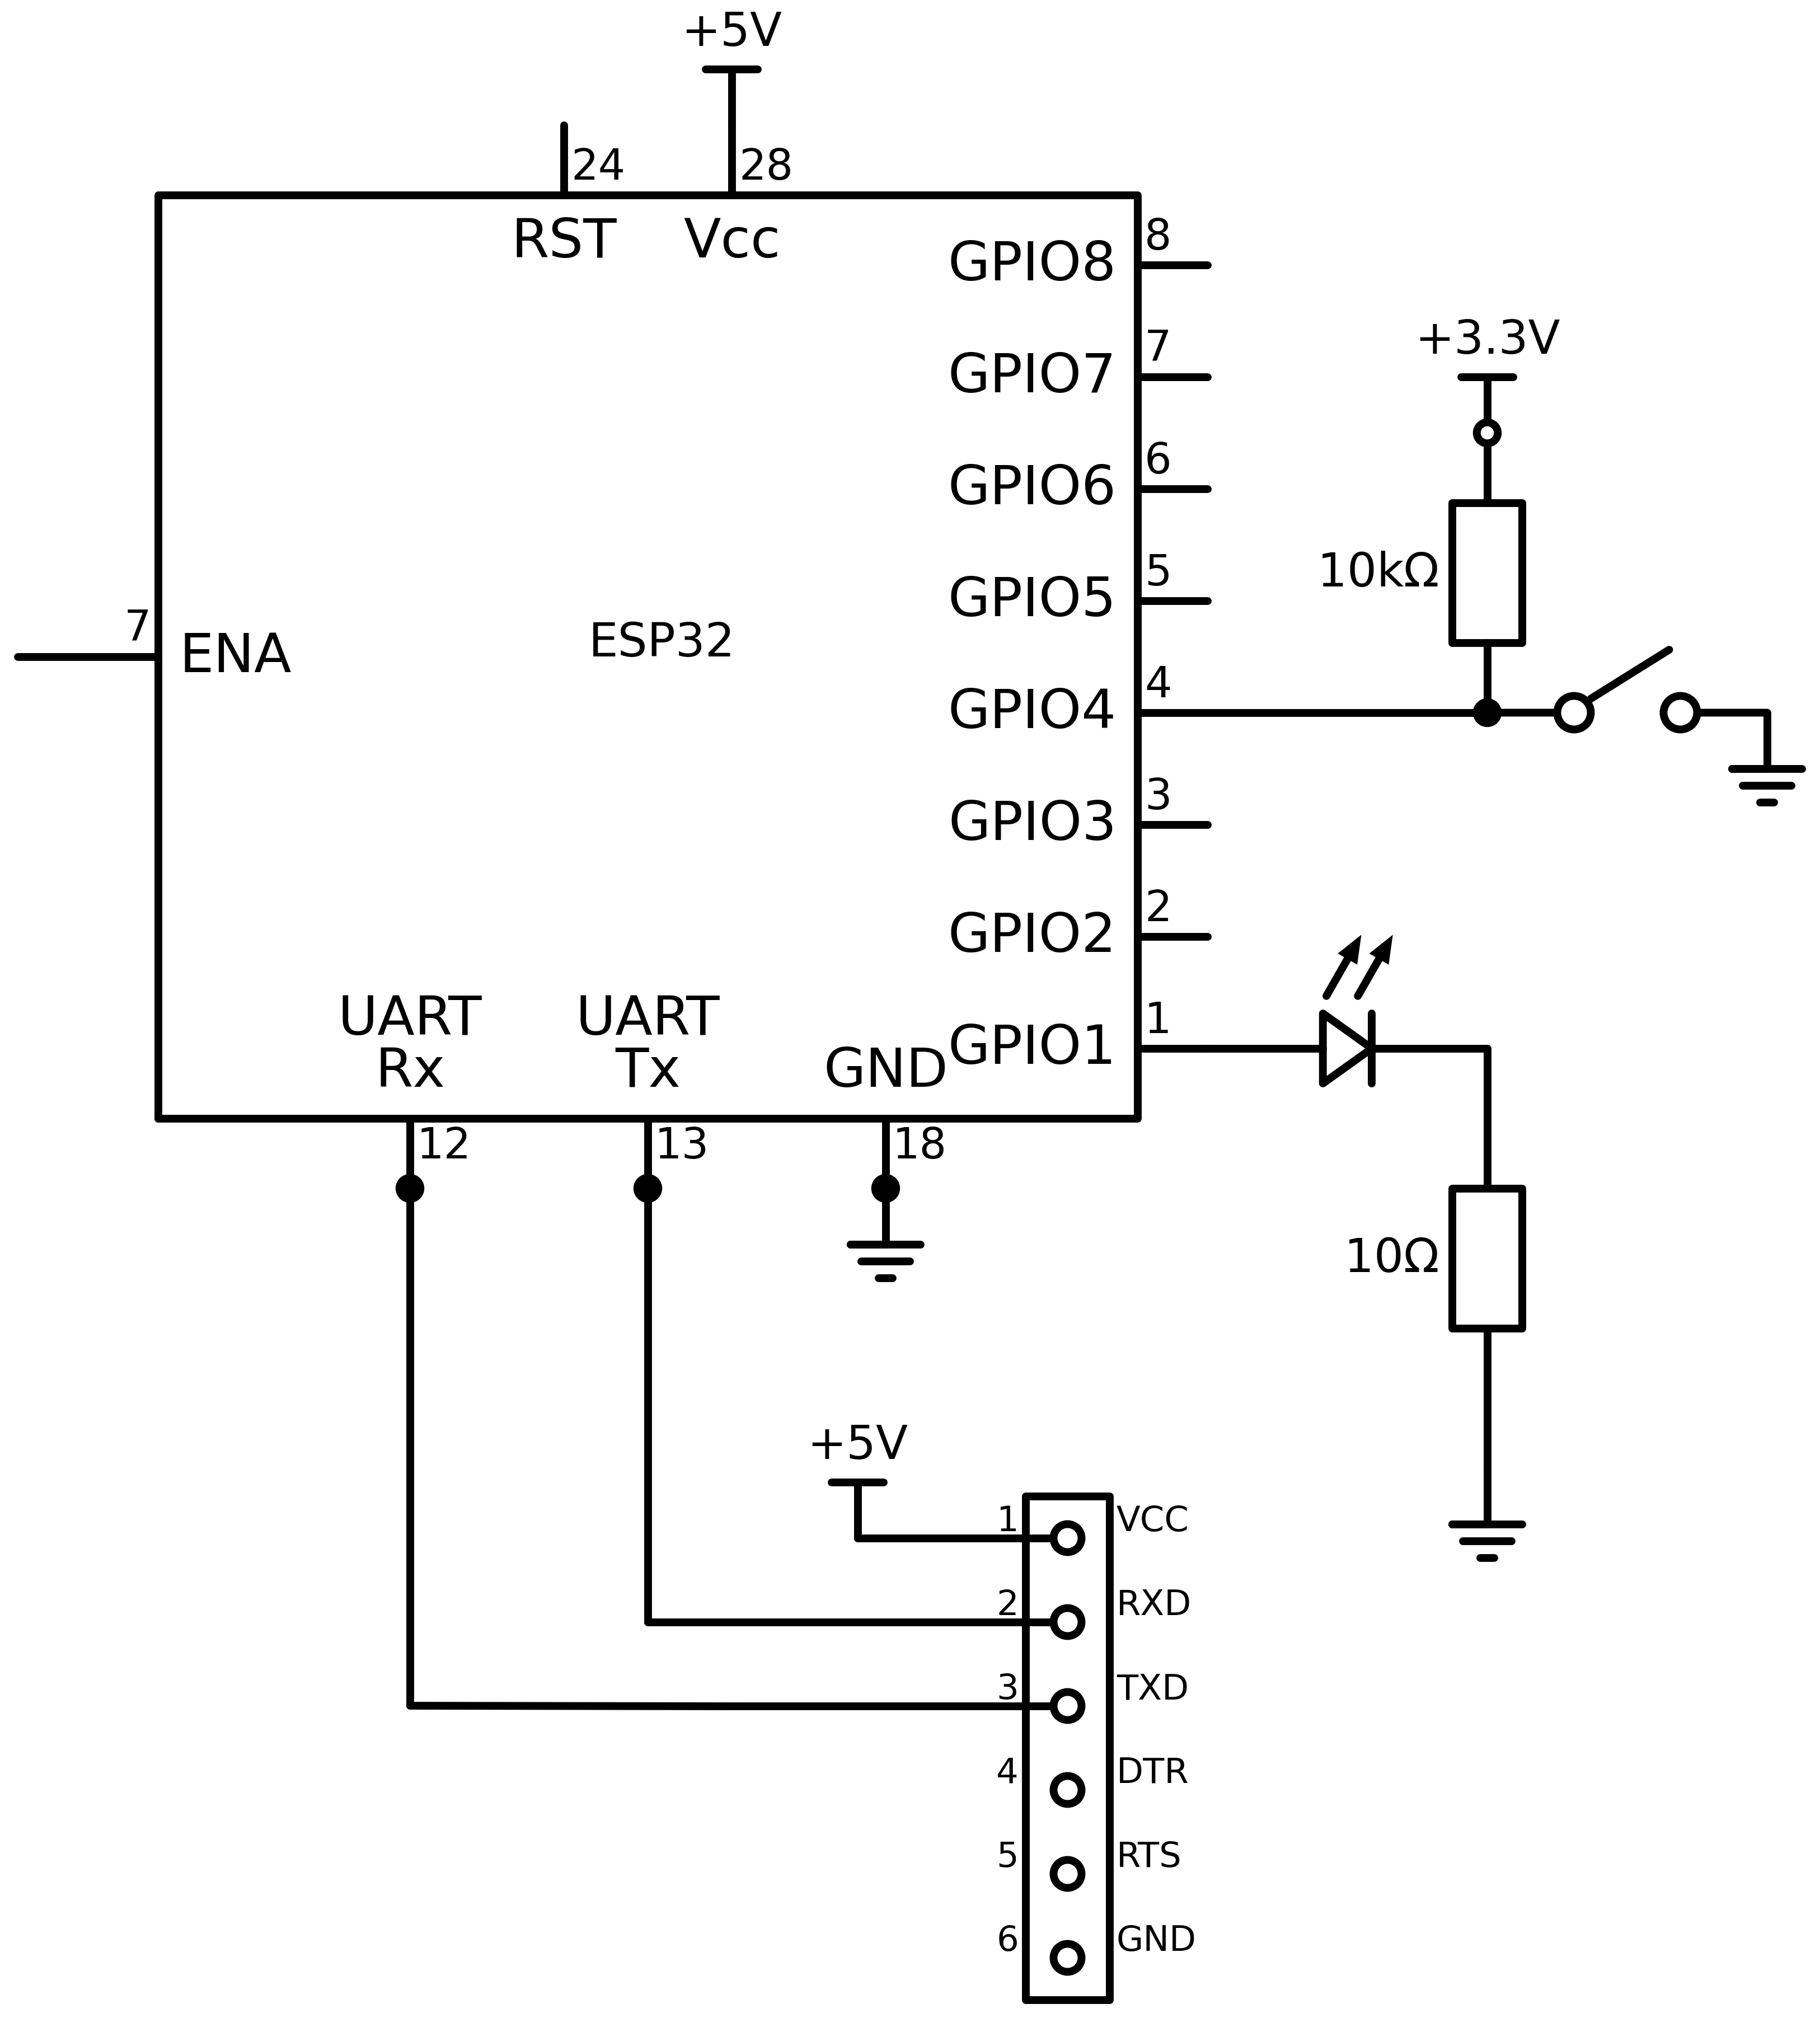
\includegraphics[width=0.9\columnwidth]{schematic.png}
  \caption{Example Schematic generated with Schemdraw \cite{schem}\label{schematic}.}
  \label{Fig:schematics}
\end{figure}

\subsection{Acknowledgments}

\noindent Acknowledgments: Those whom advice has been taken from (other than the authors) and in case results are shared with other
developers, these people should also be named and their contributions should be
acknowledged.
Acknowledgments do not diminish the value of your own work. On the contrary: They show that you have also exchanged ideas with other experts about the solution approaches and the technologies used.


\section{Before Submitting}

\noindent Before submitting your report, read it again considering the following points:

\begin{itemize}
\item Are title and abstract appropriate and do they motivate to read the paper?
\item Research: Are proper references to related work contained?
\item Technical correctness: Are the descriptions complete and free of errors? Is the presentation in scientific notation with proper units? 
\item Reproducibility: Is it possible to reproduce the results from the information given?
\item Contribution: Does the paper contain authentic examples and evaluations?
\item Readability: Is the paper well written and easy to understand?
\item Length: Is the length justified by the technical contribution?
\item Overall Impression: Does it comply with formal criteria (language, references to figures and literature, structure, completeness, etc.)? Is it easy to read and understand?
\item Check for typos and further issues.
\end{itemize}

\section{Conclusions}

\noindent By following these guidelines, you can ensure that your report is well-written and adheres to scientific standards. This approach will help the readers to clearly understand your ideas, implementations and contributions. Consequently, this will enhance the quality of your submission and potentially result in a higher grade.

\section{Acknowledgments}
This text is based on the original "Report Submission Guidelines for BIP Project" (Jan. 2025), by S.F. Peik (HSB), F. Martins (Hanze), J. Lima (IPB), Â. Ferreira (IPB), and M. Hering-Bertram (HSB). Content in Section~\ref{sec:Content} is based on the proposal made by Gijs van der Schot.

\begin{thebibliography}{20} % Breite für die Nummern
\bibitem{Dyn87}
Nira Dyn, David Levin and John A. Gregory, 
{\it A 4-point interpolatory subdivision scheme for curve design}, 
Computer Aided Geometric Design, vol. 4, no. 4, Elsevier, 1987, pp. 257-268.
\bibitem{Far02} 
Gerald Farin, {\it Curves and Surfaces for CAGD. A practical guide.}
5. Auflage, Academic Press, San Diego 2002, ISBN 1-55860-737-4
\bibitem{Lev44}
Kenneth Levenberg {\it A Method for the Solution of Certain Problems in Least Squares},
Quarterly of Applied Mathematics, vol. 2, no. 2, American Mathematical Society (AMS), 1944, pp. 164-168.
{\tt https://www.ams.org/journals/qam/1944-02-02/home.html}
\bibitem{Mar63}
Donald W. Marquardt, {\it An Algorithm for Least-Squares Estimation of Nonlinear Parameters},
SIAM Journal on Applied Mathematics, vol. 11, no. 2, Society for Industrial and Applied Mathematics
(SIAM), 1963, pp. 431-441.
{\tt https://epubs.siam.org/doi/abs/10.1137/0111030}
\bibitem{Zob14} Justin Zobel, Writing for Computer Science, 3rd edition,
Springer, 2014.
\bibitem{joke} Robot jokes, https://jokes.scoutlife.org/topics/robot-jokes/, accessed 6.1.2025
\bibitem{schem} Collin J. Delker, Schemdraw, \url{https://pypi.org/project/schemdraw/}
\end{thebibliography}

\end{document}